\section{Aufbau und Organisation des Dashboards}

\subsection{\{Golem\}}\label{chap:Golem}
\{Golem\} ist ein R-Paket, welches es erleichtert skalierbare und standardisierte Shiny-Applikationen zu bauen. Es ist Teil des golemverse und seit dem 05 August 2019 auf dem \glqq Comprehensive R Archive Network\grqq{} (CRAN) \nomenclature{\(CRAN\)}{Comprehensive R Archive Networks} gehosted \citep{ThinkR2019}.\newline
Das golemverse \citep{ThinkRnodate} ist eine Sammlung verschiedener R-Pakete, welche die Entwicklung von Shiny Dashboards beschleunigen sollen. Es wurde von dem französischen Consulting Unternehmen ThinkR \citep{Breizhtormnodate} entwickelt.\newline
ThinkR ist ein Consulting Unternehmen, welches sich auf das Ausrichten von interaktiven Trainings im Bereich der R Programmierung, mit einem Fokus auf die Entwicklung von Shiny Dashboards, spezialisiert hat. \newline
{Golem} folgt dem Grundatz \glqq convention over configuration\grqq{}. 
Einem Softwaredesign-Paradigma, welches in seiner Grundidee von David Heinemeier Hansson \citep{Hansson2016} für das Web-Framework \glqq Ruby on Rails\grqq{} entwickelt wurde. Dabei steht im Zentrum des Paradigmas die Idee, mit Konventionen die Anzahl der Entscheidungen, die ein Programmierer zu treffen hat, zu reduzieren. Dies führt zu einer hohen Softwarequalität, bei veringertem Aufwand für den Programmierer. \newline
In \{golem\} wird das durch eine vordefinierte Ordnerstruktur, zentrale Konfigurationsdateien und Funktionen zum Erstellen neuer Teile des Dashboards umgesetzt. \newline 
Dieser Ansatz hat den Vorteil, dass er das Team zu einer hohen Softwarequalität zwingt. \newline 
Im Folgenden, sollen die einzelnen Komponenten von \{golem\} näher erläutert und deren Wichtigkeit herausgestellt werden.

\begin{figure}
 \centering
 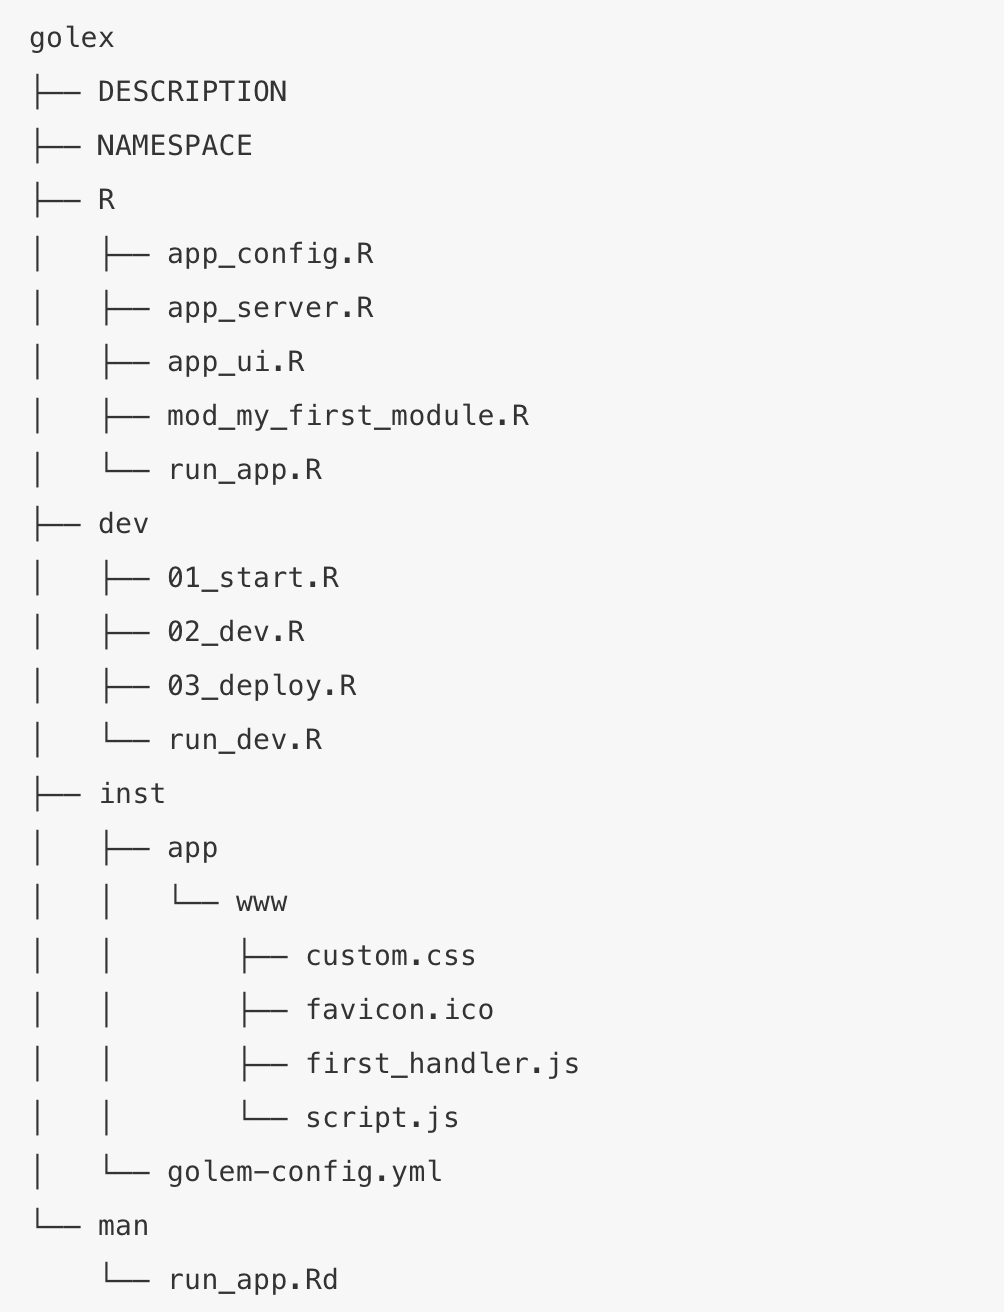
\includegraphics[scale=.4]{"images/02_Aufbau_und_Organisation/golem_app_structure.png"}
 \caption{Golem App Struktur}
\end{figure}

\subsubsection{DESCRIPTION und NAMESPACE}
Die DESCRIPTION und NAMESPACE Dateien enthalten Metadaten über das Package und sind nicht \{golem\} spezifisch.\newline 
Bei der Erstellung eines \{golem\} Projekts werden diese Dateien automatisch generiert und in der Regel bedarf es keiner manuellen Änderungen. \newline
Die DESCRIPTION Datei enthält dabei unter Anderem Daten über die Funktionen des Packages, die Lizenz, die Autoren etc.. \newline
Die NAMESPACE Datei definiert wie Interaktionen mit anderen Paketen aussehen. Dabei wird betrachtet, welche Funktionen von dem Package importiert und exportiert werden.\newline
Um eine lückenlose Dokumentation zu gewährleisten und mögliche Fehler zu vermeiden, sollte diese Datei niemals per Hand bearbeitet werden. Um Änderungen an der Datei vorzunehmen, kann das Paket \emph{attachment} \citep{Rochette2021} verwendet werden. Dieses updated, basierend auf \emph{@import} und \emph{@export} Tags in den Docstrings der einzelnen Funktionen und Modulen, die NAMESPACE Datei.
Ein solches Update kann manuell mit folgendem Command getriggert werden:
\begin{lstlisting}
attachment::att_amend_desc()
\end{lstlisting}

\subsubsection{R/}
Dieser Ordner enthält den Kern-Quellcode einer \{golem\} Applikation. 
Nach der initialen Erstellung eines \{golem\} Projekts, befinden sich vier Dateien in dem Ordner: app\_config.R, app.R, ui.R und server.R. \newline 
Die app\_config.R Datei ist \{golem\} spezifisch und enthält Konfigurationsparameter.\newline 
Die app.R Datei führt die Server-und die Ui-Funktionen zu einem Dashboard zusammen und enthält zudem \{golem\} spezifische Funktionsaufrufe. \newline 
Die ui.R Datei enthält die Definition des User-Interface der Applikation und die server.R Datei definiert die Backend-Logik, welche auf dem Server und nicht im Browser läuft.

\subsubsection{dev/}
Der dev Ordner enthält \{golem\} spezifische Utility-Funktionen, welche z.B. das Deployment der App vereinfachen. Dieser Ordner enthält keinen applikationsspezifischen Code. 

\subsubsection{inst/app/www}
Der inst/app/www Ordner enthält statische Dateien, wie z.B. Bilder oder CSS Dateien. Alle Dateien, die in diesem Ordner abgelegt werden, stehen der Applikation bei Laufzeit zur Verfügung. 

\subsection{Aufbau des Dashboards}\label{chap:Aufbau}
 Das Shiny-Dashboard startet auf der Welcomepage, wo die vier Bereiche App Status, App Mainteners, Directions und Security and License vorgefunden werden können:
\begin{figure} [H]
 \centering
 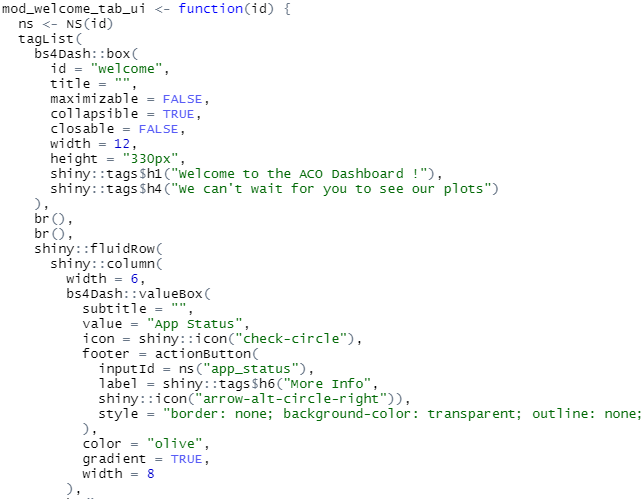
\includegraphics[scale=.8]{"images/02_Aufbau_und_Organisation/ui_welcomepage.png"}
 \caption{Quellcode des UI Funktion für die WelcomePage}
 \label{fig:fluidPage}
\end{figure}

Jeder Tab entspricht einem Shiny-Module. Diese Vorgehensweise reduziert Namespace Konflikte und entspricht den Best Practices von \{golem\}.\newline
Die Tabs selber werden in dem Dashboard auf der linken Seite abgebildet. Hierzu werden die Tabs aufgeklappt, sobald man mit dem Mauscursor über die Fläche fährt. Es gibt eine Aufteilung in Welcome, welches die WelcomePage beinhaltet, desweiteren gibt es den übergeordneten Punkt Theoretical Background, in dem die Themen Timeline, Ant Foraging und Algorithm untergebracht wurden. Der nächste übergeordnete Punkt sind Visualisations unter dem der Ant Generations Plot, Rosenbrock Plot und Himmelblau Plot vorliegt. Als letzter übergeordneter Punkt wurde Applying the algorithm verwendet, welcher das Travelling Salesman Problem und den Performancevergleich zu anderen Algorithmen beinhaltet. \newline
Die Implementierung des ACO im Algorithm Tab basiert auf dem Artikel: \glqq \emph{Ant Colony Optimization Algorithm}\grqq{} von Pablo Portillo Garrigues \citep{Garrigues2019}.